\subsection{Graph Representation}

We formulate the stablecoin cross-exchange arbitrage problem as a directed weighted graph
$G=(V,E)$. Each node $v\in V$ represents a unique stablecoin--exchange pair, written as
$v=(exchange,coin)$. Each directed edge $e\in E$ corresponds either to a trade executed on an
exchange or a transfer of funds between exchanges. 

Every edge has an associated effective exchange rate that incorporates all relevant costs---including trading fees, withdrawal fees, spreads, and slippage. We assign each edge a weight using the negative logarithm of this effective rate:
\[
w(e) = -\log\!\big(\textit{effective\_rate}(e)\big).
\] % this can be inline

This transformation converts multiplicative returns into additive costs, enabling the use of shortest-path algorithms to evaluate profitability.

\subsection{Path Profitability}

Given a path $P=(v_0,v_1,\dots,v_k)$ with initial capital $C_0$, the final capital after executing all trades and transfers along the path is
\[
C_k = C_0 \cdot \prod_{e\in P} r(e)
\]
where $r(e)$ denotes the effective rate on edge $e$. A path is profitable when the net gain exceeds a user-specified minimum profit threshold:
\[
C_k - C_0 \ge \textit{min\_profit}.
\] % this can be inline 

Expressing this condition in additive log space gives an equivalent constraint:
\[
\sum_{e\in P} -\log\!\big(r(e)\big)
\;\le\;
-\log\!\left(1+\frac{\textit{min\_profit}}{C_0}\right).
\]

Thus, the arbitrage search problem becomes the task of identifying a path that begins at a given start node $v_0$ and ends at some end node $v_k$, and yields a multiplicative return greater than one. More formally, we seek:
\[
\textit{Find } P: v_0 \to v_k \;\; \textit{s.t.}\;\; \prod_{e\in P} r(e) > 1
\]
This constitutes a minimum-cost path search under realistic execution constraints. We note that $v_k = v_0$ in standard arbitrage, but we seek the first profitable path. 

\subsection{A* Search Formulation}

To solve the arbitrage problem efficiently, we apply the A* search algorithm. For each node $n$, we maintain a cost-to-reach value $g(n)$, computed as the sum of the additive edge costs encountered so far:
\[
g(n) = \sum_{e\in path} -\log\!\big(r(e)\big).
\]

We define a heuristic function $h(n)$ that estimates the remaining cost or execution risk required to complete a profitable cycle. The A* evaluation function is given by
\[
f(n) = g(n) + h(n),
\]
where $g(n)$ denotes the accumulated path cost in log space and $h(n)$ estimates the remaining cost to complete a feasible arbitrage path. The algorithm terminates when a path yields final capital exceeding the initial capital, that is, when $C_n > C_0$. This formulation allows A* to balance realized execution costs with heuristic estimates of remaining feasibility and risk.

To never overestimate the actual cost, the heuristic satisfies the admissibility condition:
\[
h(n) \leq h^*(n),
\]
where $h(n)$ is the heuristic calculation at time of execution and $h^*(n)$ is the calculated value of the heuristic during pathfinding from node $n$ to the next node $n+1$. Since an edge's true cost is $g(n)$, calculated at time of execution, and $h(n) \geq 0$, our A* formulation remains admissible under the condition that path node cost remains constant at execution.

For search efficiency, the heuristic should also satisfy the consistency condition:
\[
h(n) \leq c(n, n') + h(n'),
\]
where $c(n, n')$ is the transition cost between adjacent nodes $n$ and $n'$. This condition implies that the $f$-value does not decrease along a path, ensuring that nodes do not require re-expansion once visited.

Lastly, we note that the algorithm is not complete as market data never guarantees a profitable trading path for all starting exchange nodes $v\in V$.


\subsection{Demonstrative Example}

Consider a simplified arbitrage graph with three nodes: $\text{binance:USDT}$, $\text{kucoin:USDT}$, and $\text{kucoin:TUSD}$. Suppose we have the following edges with effective rates:

\begin{itemize}
\item $\text{binance:USDT} \to \text{kucoin:USDT}$: rate $r_1 = 0.9995$ (includes transfer fee)
\item $\text{kucoin:USDT} \to \text{kucoin:TUSD}$: rate $r_2 = 1.0042$ (profitable trade)
\item $\text{kucoin:TUSD} \to \text{binance:USDT}$: rate $r_3 = 0.9995$ (transfer back)
\end{itemize}

\begin{figure}[t]
    \centering
    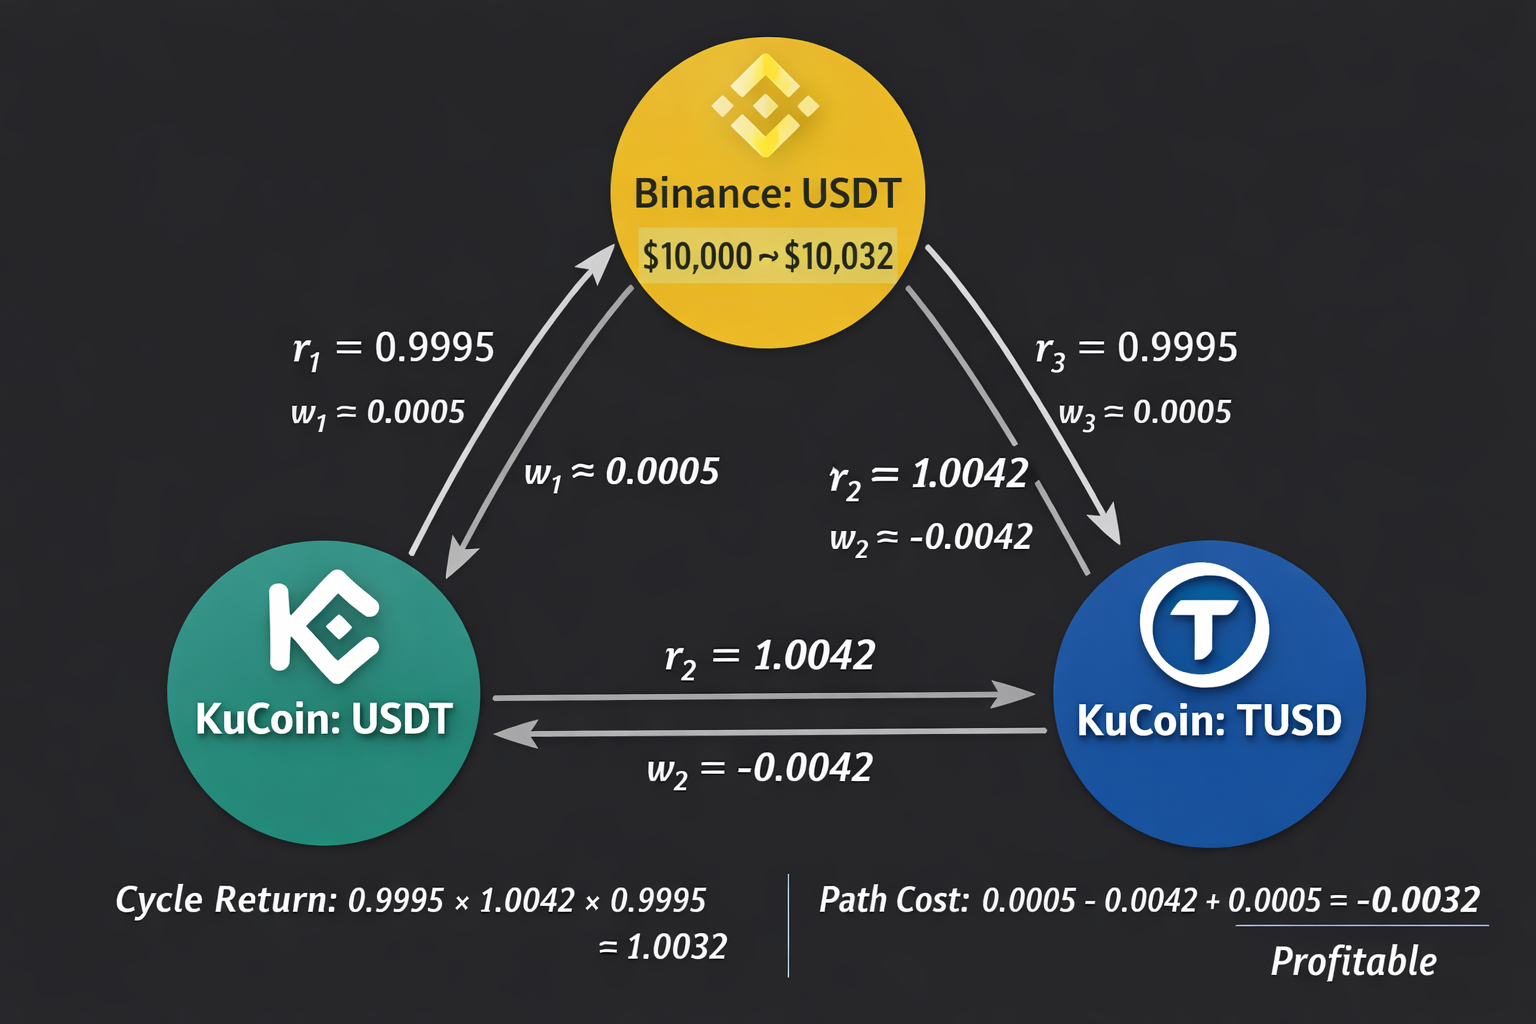
\includegraphics[width=0.9\linewidth]{figures/arbitrage_path.png}
    \caption{
    Simplified three-node arbitrage cycle across Binance and KuCoin.
    Edge labels denote effective multiplicative rates $r_i$ and corresponding
    log-space weights $w_i = -\log r_i$. The total log-cost of the cycle is
    negative, indicating a theoretical profitable arbitrage opportunity. It is important to note, our research is not constrained to profitable cycles, and is allows for any profitable path to represent a goal state.
    }
    \label{fig:arbitrage_example}
\end{figure}


The cycle $\text{binance:USDT} \to \text{kucoin:USDT} \to \text{kucoin:TUSD} \to \text{binance:USDT}$ has a multiplicative return of:
\[
\prod_{e\in P} r(e) = 0.9995 \times 1.0042 \times 0.9995 \approx 1.0032
\]

Starting with \$10,000, the final capital would be approximately \$10,032, yielding a profit of \$32. The edge weights in log space are:
\begin{align}
w_1 &= -\log(0.9995) \approx 0.0005 \\
w_2 &= -\log(1.0042) \approx -0.0042 \\
w_3 &= -\log(0.9995) \approx 0.0005
\end{align}

The total path cost is $0.0005 - 0.0042 + 0.0005 = -0.0032$, which is negative, indicating a profitable cycle (negative cost in log space corresponds to positive return).